\newpage

\section[Обзор предметной области]{\large \centering Обзор предметной области}
\hspace{\parindent} Выравнивание аминокислотных или нуклеотидных последовательностей --- это процесс сопоставления сравниваемых последовательностей для такого их взаиморасположения, при котором наблюдается максимальное количество совпадений аминокислотных остатков или нуклеотидов~\cite{AlignmentClustal}. Различают два вида выравнивания: парное (выравнивание двух последовательностей ДНК, РНК или белков) и множественное (выравнивание трех и более последовательностей). 

\subsection[Существующие методы поиска гомологий в биологических последовательностях]{\large Существующие методы поиска гомологий в биологических последовательностях} \label{sec:SearchHmlg}
\hspace{\parindent} В генетике под гомологиями понимаются участки белков или ДНК, имеющие сходную последовательность аминокислот или нуклеотидов. Обычно существа, у которых есть гомологичные участки белков или ДНК, имеют общего предка, от которого они и получили такой участок. Поскольку в процессе эволюции ДНК подвергается мутациям, эти участки не обязательно идентичны. В них могут быть случайно заменены, добавлены или удалены нуклеотиды или аминокислоты (рисунок~\ref{ris:Mutation}). Некоторые мутации, такие, как транслокации и инверсии, приводят к изменениям, затрагивающим большие участки генома. Такие мутации сложно учитывать, поскольку локальное сходство проверять легче, чем глобальное, а в результате глобальных мутаций участки ДНК могут быть соединены в непредсказуемом порядке. %Поэтому существующие методы поиска гомологий умеют находить участки (подстроки) двух последовательностей, которые отличаются не очень сильно.

\begin{figure}[h]
	\center{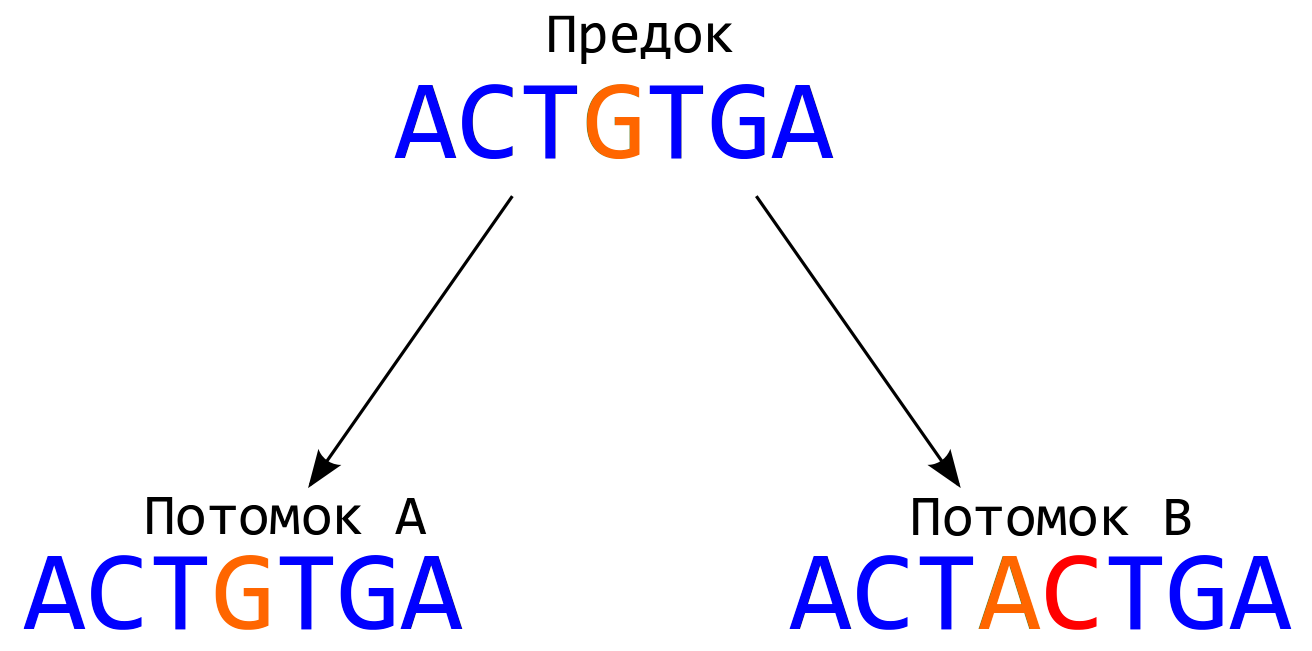
\includegraphics[width=0.60\linewidth]{transform.png}}
	\caption{Пример мутации}
	\label{ris:Mutation}
\end{figure}

\subsubsection[Алгоритм Нидлмана-Вунша]{\large Алгоритм Нидлмана-Вунша} \label{seq:NW}
\hspace{\parindent} Одним из наиболее распространенных алгоритмов выравнивания является алгоритм Нидлмана-Вунша~\cite{NWalgo}, основанный на двумерном динамическом программировании. Для своей работы алгоритм использует матрицу сходства, которая указывает, насколько схожими можно считать разные нуклеотиды. Использование матрицы позволяет придавать разный вес разным заменам нуклеотидов. Например, поскольку транзиции более вероятны, чем трансверсии, логично считать последовательности, отличающиеся заменой пурина на пурин или пиримидина на пиримидин, более схожими, чем те, которые отличаются заменой пурина на пиримидин или наоборот. Обычно используется симметричная матрица, однако, применение несимметричной матрицы позволяет различать замены в одну и в другую стороны. На рисунке~\ref{ris:ReplaceMatrix} представлен пример матрицы сходства. Здесь А, Г, Т и Ц обозначают, соответственно, аденин, гуанин, тимин и цитозин, а числа в матрице указывают степень сходства между двумя нуклеотидами.

\begin{figure}[h]
	\center{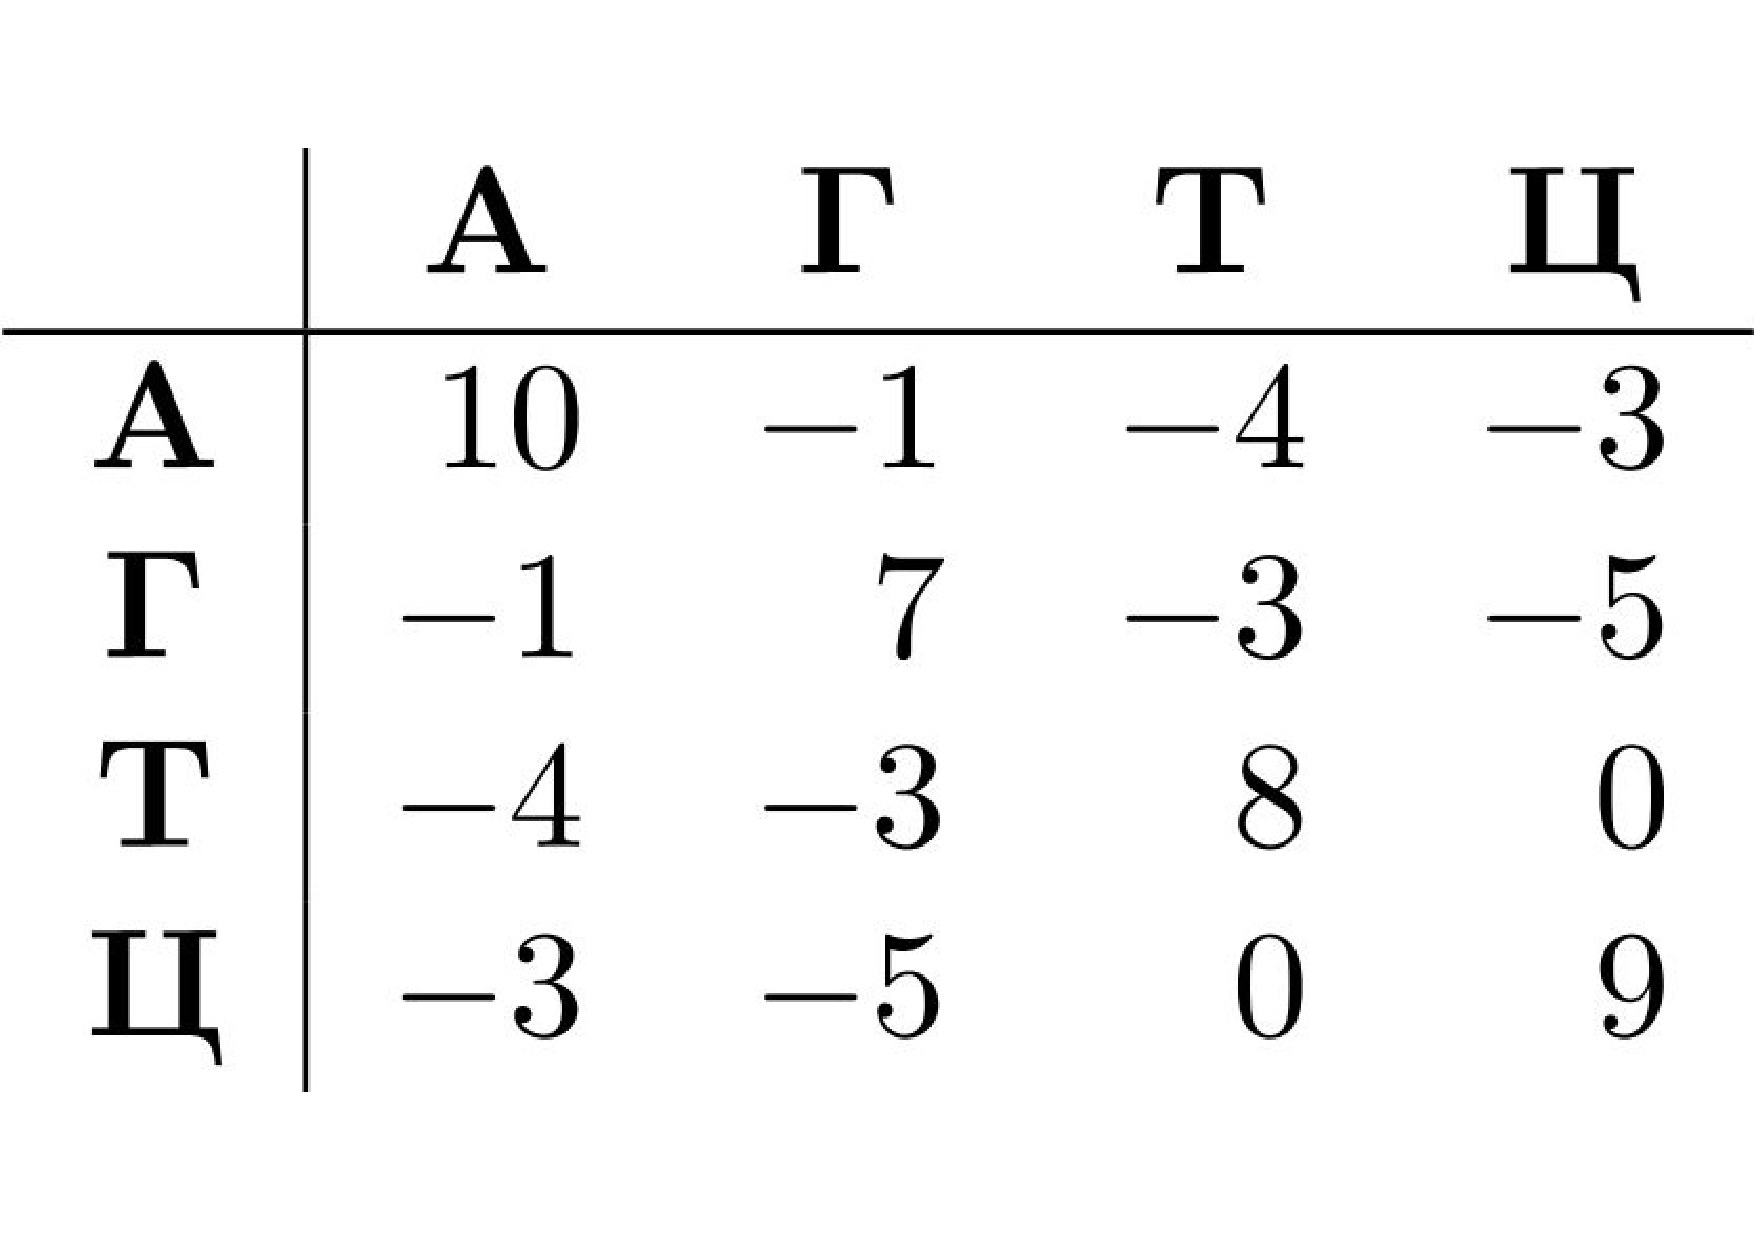
\includegraphics[width=0.35\linewidth]{RM.pdf}}
	\caption{Пример матрицы сходства}
	\label{ris:ReplaceMatrix}
\end{figure}

\indent Еще один параметр алгоритма --- штраф за разрыв последовательности. Он может выражаться произвольной функцией от длины и/или направления разрыва. Для определенности будем рассматривать линейный штраф за разрыв, определяющийся параметром $d$ (за разрыв длинны $n$ будет начислен штраф $d \cdot n$).\\
\indent На вход алгоритм получает матрицу сходства $S$, параметр штрафа $d$ и две последовательности (строки), которые необходимо выровнять. Для получения результата выполняется построение матрицы $F_{i,j}$ , где $i$ и $j$ изменяются от нуля до длины, соответственно, первой и второй строк. Вначале алгоритм инициализирует $F_{i,0}$ и $F_{0,j}$ равными, соответственно, $d \cdot i$ и $d \cdot j$ для всех $i$ и $j$. Затем происходит вычисление оставшихся элементов матрицы по формуле~\ref{eq:N_W}.

\begin{equation}\label{eq:N_W}
F_{i,j} = max\left\{
	\begin{aligned}
		& F_{i-1,j-1} + S_{A_i,B_j}\\
		& F_{i-1,j} + d\\
		& F_{i,j-1} + d
	\end{aligned}
	\right.
\end{equation}

\indent  После того как матрица посчитана, необходимо определить, каким путем появилось значение в правом нижнем углу. Например, если $F_{i,j} = F_{i-1,j-1} +S_{A_{i-1},B_{j-1}}$, то элемент $(i, j)$ появился из элемента $(i - 1, j - 1)$, и т. д. Элементы в верхней строке произошли из элементов левее себя, элементы из левого столбца --- из элементов выше себя. Переход вида $(i, j) \rightarrow (i - 1, j - 1)$ означает, что $i$-му символу в первой строке соответствует $j$-й символ во второй строке. Переход вида $(i, j) \rightarrow (i - 1, j)$ означает, что $i$-му символу первой строки ничего не соответствует, а переход $(i, j) \rightarrow (i, j - 1)$ --- что $j$-му символу второй строки ничего не соответствует. Путь в матрице от левого верхнего угла к правому нижнему даст искомое выравнивание последовательностей.\\
\indent Очевидно, что алгоритм всегда ищет выравнивание с максимальным счетом, так как, строя матрицу $F$, он рассматривает всевозможные варианты размещения одной строки относительно другой. Время работы и количество используемой памяти пропорционально произведению длин последовательностей.

\subsubsection[Алгоритм Смита-Ватермана]{\large Алгоритм Смита-Ватермана}
\hspace{\parindent} Алгоритм Смита-Ватермана~\cite{SWalgo} аналогичен алгоритму Нидлмана-Вунша, но решает задачу локального выравнивания: находит подстроки первой и второй строк, обладающие максимальным сходством.\\
\indent На вход алгоритм получает матрицу сходства $S$, две последовательности и два вектора $I$ и $D$, вектор стоимостей добавления и вектор стоимостей удаления, соответственно. Элементы матрицы $F_{i,0}$ и $F_{0,j}$ инициализируются нулями.  Вычисление оставшихся элементов происходит по формуле~\ref{eq:S_W}.

\begin{equation}\label{eq:S_W}
F_{i,j} = max\left\{
	\begin{aligned}
		& F_{i-1,j-1} + S_{A_i,B_j}\\
		& F_{i-1,j} + D_{A_i}\\
		& F_{i,j-1} + I_{B_j}\\
		& 0
	\end{aligned}
	\right.
\end{equation}

\indent Для получения выравнивания необходимо найти максимальный элемент в матрице. Если переходить от этого элемента по цепочке предыдущих, то путь закончится в каком-то нулевом элементе. Индексы этих двух элементов равны индексам начал и концов подстрок: первые индексы --- в первой строке, вторые --- во второй. Путь интерпретируется так же, как и в алгоритме Нидлмана-Вунша.\\
\indent Видно, что оба алгоритма похожи друг на друга. Они имеют одинаковую сложность и затраты по памяти, что делает такие алгоритмы неприемлемыми для работы с большим количеством генетического материала.

\subsubsection[Алгоритм Хиршберга]{\large Алгоритм Хиршберга}
\hspace{\parindent} Оба предыдущих алгоритма требуют объем памяти, пропорциональный произведению длин выравниваемых последовательностей, что затрудняет обработку больших строк, поэтому очень важно иметь методы, уменьшающие затраты памяти без критического увеличения времени счета. В 1975 году был предложен алгоритм Хиршберга, значительно сокращающий затраты памяти~\cite{Hirshberg}. Он позволяет вычислять оптимальное выравнивание строк длины $n$ и $m$, используя $O(n+m)$ количество памяти, но примерно вдвое большее времени счета по сравнению с алгоритмом Нидлмана-Вунша.\\
\indent Идея алгоритма состоит в том, что одна из двух входных последовательностей разбивается на две части, и исходная задача сводится к двум, меньшим, задачам выравнивания второй входной последовательности с каждой из частей. Решение подзадач осуществляется путем аналогичного сведения к подзадачам. На рисунке~\ref{ris:Hirshberg} показана схема разбивки задачи на две подзадачи: верхнюю, которая решается в прямоугольнике $A$ исходной таблицы, и нижнюю --- в прямоугольнике $B$. Последовательности имеют длины $n$ и $m$, соответственно. Для разбиения каждой задачи на подзадачи необходимо вычислить значение $k^*$. При этом используется объем памяти, линейно зависящий от $m$. Верхняя задача заключается в выравнивании строки с длинами не больше $n/2$ и $k^*$, а нижняя – с длинами не больше $n/2$ и $m-k^*$. 

\begin{figure}[h]
	\center{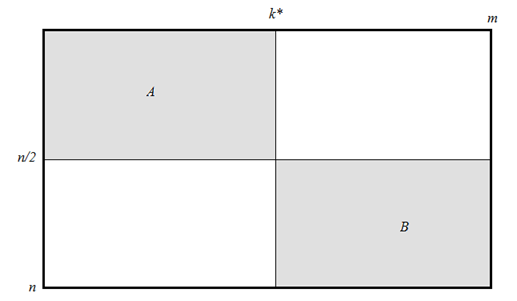
\includegraphics[width=0.7\linewidth]{hirshberg.png}}
	\caption{Разделение задачи выравнивания на две подзадачи}
	\label{ris:Hirshberg}
\end{figure}

\indent Для представления задач в алгоритме Хиршберга можно использовать бинарные деревья~\cite{HirshbergParallel}. Узлам дерева соответствуют подзадачи, которые заключаются в выравнивании меньших подпоследовательностей. Каждый узел дерева хранит в памяти границу прямоугольной области, в которой решается соответствующая задача динамического программирования. Дерево в процессе работы алгоритма строится по уровням. Сначала оно состоит только из корневого узла, который соответствует прямоугольнику $[0,0]\times[n,m]$. Создание двух узлов эквивалентно разбиению задачи на две подзадачи и разделению области решения на две, меньшего размера.\\
\indent Алгоритм Хиршберга заключается в обходе полного дерева всех подзадач. Результат выравнивания можно будет получить, если пройтись по листьям построенного дерева (рисунок~\ref{ris:HirshbergExample}). Для оптимизации вычислений можно выполнять обход (решение подзадач) только части вершин дерева: тех, которые удалены от корня на величину, не превосходящую заранее заданную константу $h$ --- максимальную глубину обхода дерева. При достижении глубины дерева $h$ или минимального размера прямоугольника применяется алгоритм Нидлмана-Вунша, который работает вдвое быстрее алгоритма Хиршберга.

\begin{figure}[h]
	\center{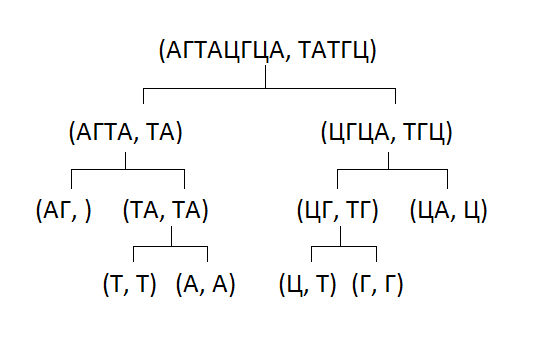
\includegraphics[width=0.7\linewidth]{hirshberg-example.png}}
	\caption{Дерево подзадач для алгоритма Хиршберга}
	\label{ris:HirshbergExample}
\end{figure}

\indent Дополнительное ускорение можно получить за счет распараллеливания. Заметим, что на каждом шаге алгоритма полученные подзадачи никак не связаны между собой, и, следовательно, их решения могут вычисляться в отдельных потоках.

\subsection[Алгоритмы множественного выравнивания]{\large Алгоритмы множественного выравнивания} \label{sec:Multy}
\hspace{\parindent} В пункте~\ref{sec:SearchHmlg} были рассмотрены основные подходы для получения парного выравнивания. Для некоторых областей биоинформатики задачу поиска выравнивания необходимо переложить на многомерный случай, например, при реконструкции эволюционной последовательности (получение филогенетических деревьев) или при выявлении шаблона функциональных семейств и сигналов ДНК.

\subsubsection[Выравнивание в <<кубе>>]{\large Выравнивание в <<кубе>>}
\hspace{\parindent} Рассмотрим задачу выравнивания трех последовательностей: $A_1$, $A_2$ и $A_3$. Построим трехмерную матрицу $F$ (рисунок~\ref{ris:Cube}) с длинами сторон $len(A_i)$, $i = 1,2,3$, где $len(A_i)$ --- длина $i$-ой строки. Аналогично алгоритму Нидлмана-Вунша (пункт~\ref{seq:NW}) определим значение в ячейке $F_{i,j,k}$ $i=1 \ldots len(A_1)$, $j=1 \ldots len(A_2)$, $k=1 \ldots len(A_3)$ по формуле~\ref{eq:CubeAlign}.

\begin{figure}[h]
	\center{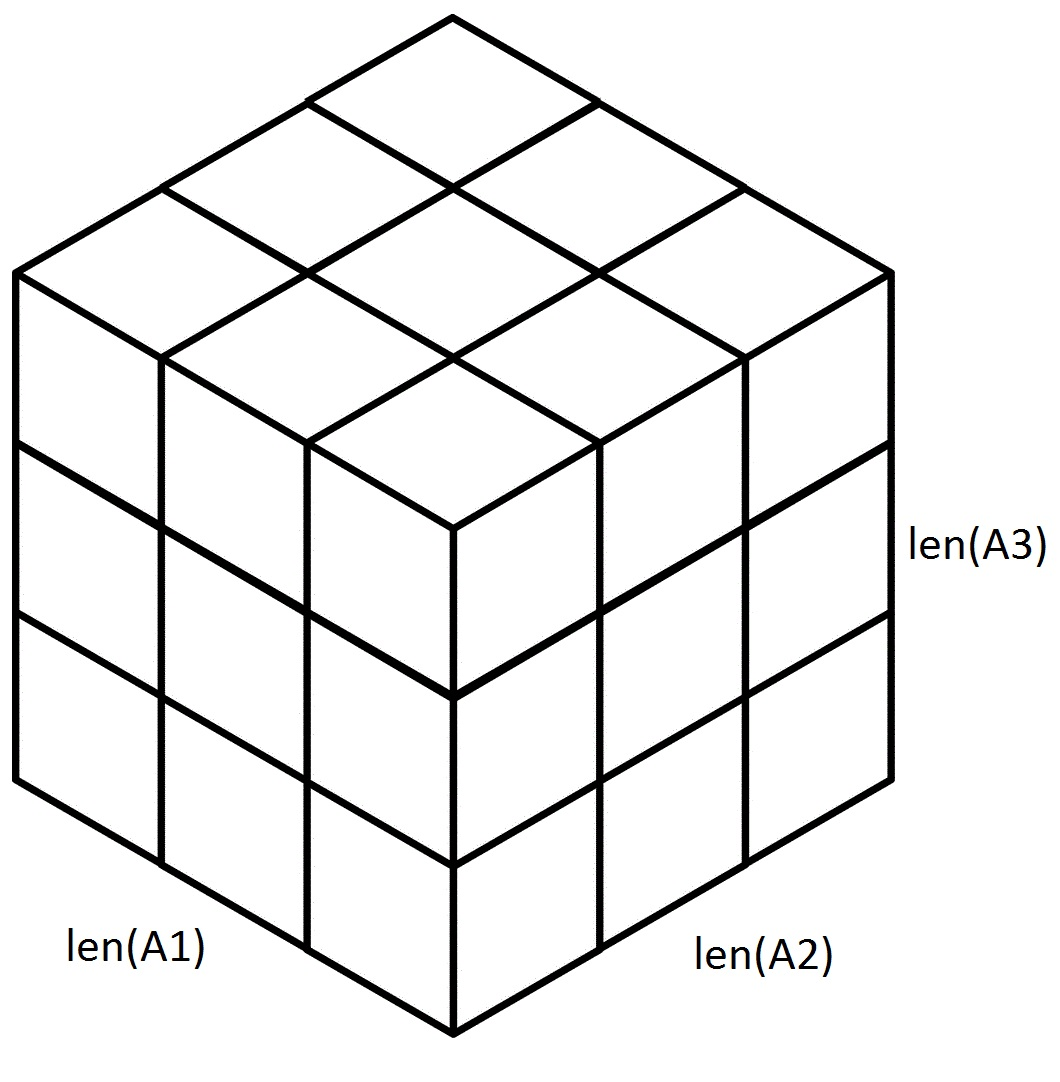
\includegraphics[width=0.35\linewidth]{cube.jpg}}
	\caption{Матрица $F$ для выравнивания трех последовательностей}
	\label{ris:Cube}
\end{figure}

\begin{equation}\label{eq:CubeAlign}
F_{i,j,k} = max\left\{
	\begin{aligned}
		& F_{i-1,j-1,k-1} + S(A_{1_i},A_{2_j}) + S(A_{1_i},A_{3_k}) + S(A_{2_j},A_{3_k})\\
		& F_{i-1,j-1,k} + S(A_{1_i},A_{2_j}) + 2d\\
		& F_{i-1,j,k-1} + S(A_{1_i},A_{3_k}) + 2d\\
		& F_{i,j-1,k-1} + S(A_{2_j},A_{3_k}) + 2d\\
		& F_{i-1,j,k} + 3d\\
		& F_{i,j-1,k} + 3d\\
		& F_{i,j,k-1} + 3d\\
	\end{aligned}
	\right.
\end{equation}

\indent Можно заметить, что каждая грань куба --- это парное выравнивание двух последовательностей с учетом некоторой части третьей, что и дает в итоге полный перебор всех возможных вариантов. Нулевые грани куба $F_{0,j,k}$, $F_{i,0,k}$ и $F_{i,j,0}$ заполняются аналогично алгоритму Нидлмана-Вунша.

\indent  Чтобы получить ответ, необходимо найти путь от ячейки $F_{len(A_1),len(A_2),len(A_3)}$, где записан итоговый счет за выравнивание, до $F_{0,0,0}$. Так как имеется всего семь возможных перемещений в кубе и $len(A_1) \cdot len(A_2) \cdot len(A_3)$ ячеек, то сложность алгоритма можно оценить как $O(7\prod\limits_{i=1}^3len(A_i))$.

\indent Не составляет большого труда <<продлить>> аналогичным образом это решение на $n$-мерный случай и получить <<честное>> многомерное выравнивание. Под словом <<честное>> подразумевается, что рассмотрены все возможные варианты выравнивания последовательностей, и полученный результат всегда имеет максимальный счет. Единственный недостаток --- слишком большая вычислительная сложность алгоритма: $O((2^n-1)\prod\limits_{i=1}^nlen(A_i))$, что делает такой подход совершенно неприменимым для выравнивания большого числа и/или длинных последовательностей. 

\subsubsection[Выравнивание выравниваний. Алгоритм Clustal]{\large Выравнивание выравниваний. Алгоритм Clustal}\label{align-align}
\hspace{\parindent} Другой подход заключается в получении парного выравнивания между первыми двумя последовательностями, после чего полученный результат выравнивается с третьей и так далее. То есть, если $f$ --- функция вычисления парного выравнивания, а $A_1, \ldots ,A_n$ --- выравниваемые последовательности, то алгоритм можно условно записать формулой~\ref{eq:Closure}.

\begin{equation}\label{eq:Closure}
f(f(f(\ldots f(f(A_1, A_2), A_3) \ldots ), A_{n-1}), A_n)
\end{equation} 

\indent Очевидно, что результат алгоритма будет зависеть от порядка исходных последовательностей. Существуют различные соображения по поводу наиболее правильного выбора этого порядка. Можно не ограничиваться выравниваниями типа <<последовательность против выравнивания>>, но также производить выравнивание <<выравнивание против выравнивания>>. Например, если есть четыре последовательности, из которых первая очень похожа на четвертую, вторая --- на третью, а гомология между остальными парами (1-2, 1-3, 2-4, 3-4) более слабая, то разумно сначала сделать два парных выравнивания: первой последовательности с четвертой и второй с третей, а затем уже выровнять эти два выравнивания друг с другом.

\indent Похожим образом работает Clustal --- один из самых популярных алгоритмов множественного выравнивания. По сути, это жадный алгоритм с <<умным>> способом выбора пар. Сначала происходит построение всех парных выравниваний, после чего по полученным результатам строится <<дерево-подсказка>>. На рисунке~\ref{ris:Clustal} представлен пример возможного дерева. Для четырех последовательностей $A_1, A_2, A_3$ и $A_4$ строится таблица (на рисунке слева), числа в которой обозначают их схожесть друг с другом. Видно, что самые близкие последовательности --- $A_1$ и $A_3$, и их выравнивание будет первым, затем оно выравнивается с $A_4$, а последнее --- с $A_2$.

\begin{figure}[h]
	\center{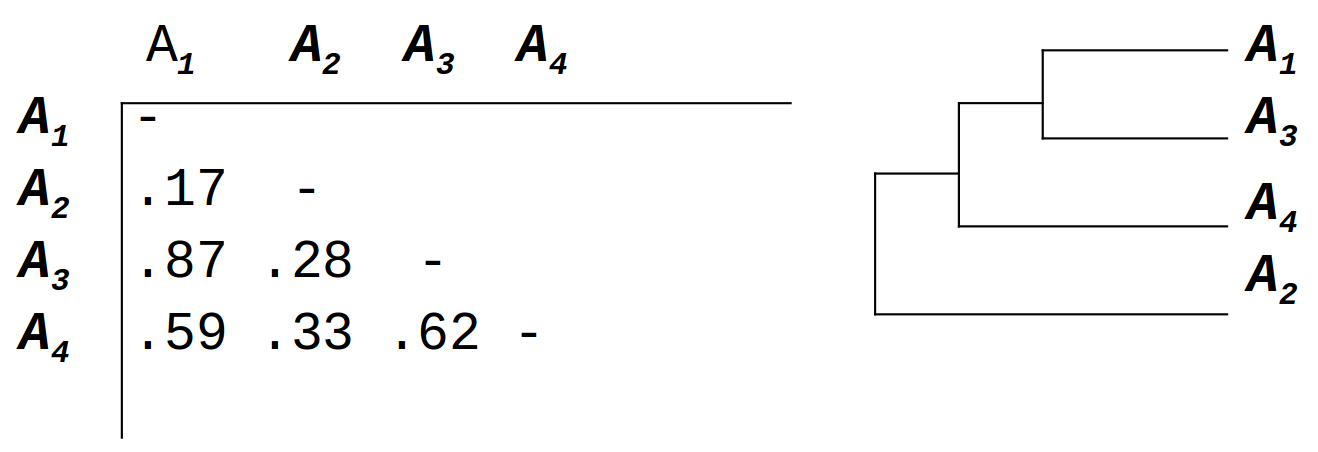
\includegraphics[width=0.79\linewidth]{Clustal.png}}
	\caption{Построение дерева-подсказки для алгоритма Clustal}
	\label{ris:Clustal}
\end{figure}

\subsection[Выравнивание с учетом открытых рамок считывания]{\large Выравнивание с учетом открытых рамок считывания}
\hspace{\parindent} Изменению числа нуклеотидных пар в цепи ДНК способствуют воздействия на генетический материал некоторых химических веществ, например акридиновых соединений~\cite{BioBook}. Деформируя структуру двойной спирали ДНК, они приводят к вставке дополнительных оснований или их выпадению при репликации. Однако, куда более вероятно возникновение ошибки на этапе секвенирования.\\
\indent Рассмотренные в пунктах~\ref{sec:SearchHmlg}~и~\ref{sec:Multy} алгоритмы множественного и парного выравниваний применимы для любых, не обязательно биологических, последовательностей, например, текстов статей или исходных кодов программ на предмет поиска плагиата. Изложенные выше методы подходят к задаче выравнивания исключительно на математическом уровне, в том плане, что они производят поиск выравнивания с максимальным счетом, совершенно не опираясь на логический смысл входных данных. Возвращаясь непосредственно к задачам биоинформатики, для поиска <<правильного>> выравнивания последовательностей необходимо использовать более сложные алгоритмы, учитывающие трансляцию полученного результата на уровень аминокислот.

\subsubsection[Трехэтапный подход]{\large Трехэтапный подход}
\hspace{\parindent} Один из самых простых способов построения <<правильного>> выравнивания --- произвести трансляцию нуклеотидной последовательности в аминокислотную по всем возможным рамкам считывания, после чего произвести выравнивание <<классическими>> алгоритмами, и, в завершение, транслировать полученный белок обратно в последовательность нуклеотидов. Для автоматизации выполнения этих трех шагов были разработаны программы revTrans~\cite{RevTrans}, transAlign~\cite{transAlign}, TranslatorX~\cite{TranslatorX} и PAL2NAL~\cite{PAL2NAL}, которая, по сравнению с остальными, дополнительно позволяет указать позиции известных рамок считывания. \\
\indent Основным недостатком этого трехступенчатого подхода является его неспособность справляться с неожиданной заменой рамки считывания. Все последующие этапы алгоритма после неправильной первой трансляции уже никак не смогут это исправить. В лучшем случае этот ошибочный перевод быстро приведет к появлению стоп-кодона, который будет сигналом для предупреждения пользователя о неправильной трансляции. В худшем случае программа построит выравнивание, которое будет очень сильно расходиться с действительностью.

\subsubsection[Двухуровневое выравнивание]{\large Двухуровневое выравнивание} \label{NTAAalign}
\hspace{\parindent} В 1994 году был предложен еще один подход для решения этой задачи. Автором была предложена модель, по которой штраф за выравнивание являлся сочетанием двух штрафов: на аминокислотном и нуклеотидном уровнях~\cite{Hein}. Он рассмотрел частный случай идеализированной эволюции исходных последовательностей, при котором инсерции допустимы только на аминокислотном уровне (запрет на сдвиг рамки считывания), а штраф за выравнивание вычислялся просто как сумма штрафов на обоих уровнях. Предложенный алгоритм выравнивания двух последовательностей длины $n$ и $m$ имел сложность $O(n^2m^2)$.\\
\indent Позже этот алгоритм был оптимизирован и перенесен на модель с аффинными штрафами и итоговой сложностью $O(nm)$~\cite{HeinOptimize}. Эти улучшения казались многообещающими, так как асимптотическая сложность алгоритма получилась точно такая же, как и у классических методов выравнивания. Однако, необходимо отметить, что постоянный множитель, спрятанный в оценке сложности $O$, ограничивает применение этого алгоритма на практике. Для получения парного выравнивания алгоритму необходимо вычислить примерно $400nm$ значений, что, к сожалению, делает его неприменимым для задачи множественного выравнивания.

\subsubsection[MACSE]{\large MACSE}
\hspace{\parindent} MACSE (Multiple Alignment of Coding SEquences Accounting for Frameshifts and Stop Codons) --- это программа для множественного выравнивания кодирующих последовательностей с учетом существующих рамок считывания и стоп-кодонов~\cite{MACSE}. Кроме задачи выравнивания, она может быть применена для обнаружения недокументированных рамок считывания в публичных базах данных.\\
\indent Алгоритм MACSE основывается на идее двухуровневого выравнивания, но требует меньше времени на вычисление парного выравнивания, благодаря чему возможно его расширение на многомерный случай. Для получения многомерного выравнивания $n$ строк $S_1 \ldots S_n$ MACSE производит выравнивание выравниваний, выбирая порядок через дерево-подсказку, как и алгоритм Clustal. 